\documentclass[10pt,twocolumn,letterpaper]{article}

\usepackage{cvpr}
\usepackage{times}
\usepackage{epsfig}
\usepackage{graphicx}
\usepackage{amsmath}
\usepackage{amssymb}
\usepackage{subcaption}

% Include other packages here, before hyperref.

% If you comment hyperref and then uncomment it, you should delete
% egpaper.aux before re-running latex.  (Or just hit 'q' on the first latex
% run, let it finish, and you should be clear).
\usepackage[breaklinks=true,bookmarks=false]{hyperref}

\cvprfinalcopy % *** Uncomment this line for the final submission

\def\cvprPaperID{****} % *** Enter the CVPR Paper ID here
\def\httilde{\mbox{\tt\raisebox{-.5ex}{\symbol{126}}}}

% Pages are numbered in submission mode, and unnumbered in camera-ready
%\ifcvprfinal\pagestyle{empty}\fi
\setcounter{page}{1}
\begin{document}

%%%%%%%%% TITLE
\title{Denoising Dirty Scanned Documents}

\author{Eric Qiu\\
University of Waterloo\\
Waterloo, ON, Canada\\
{\tt\small eric.qiu@uwaterloo.ca}
% For a paper whose authors are all at the same institution,
% omit the following lines up until the closing ``}''.
% Additional authors and addresses can be added with ``\and'',
% just like the second author.
% To save space, use either the email address or home page, not both
\and
Ooi Yuxuan\\
Nanyang Technological University\\
Singapore\\
{\tt\small OOIY0007@ntu.edu.sg}
}

\maketitle
%\thispagestyle{empty}

%%%%%%%%% ABSTRACT
\begin{abstract}
   This paper aims to provide a solution to remove unwanted background noise in a scanned document. During the first stage of training, we used different models including CNN autoencoders, median filtering, edge detection, erosion, dilation, and adaptive thresholding. We then combined the outputs of the models as inputs to a CNN stacker model to perform the second round of training. The new stacker model combines and learns the predictions of the base models to produce a better prediction.
\end{abstract}

%%%%%%%%% BODY TEXT
\section{Introduction}

    An ideal scanned document would be a clean document without being contaminated. However, we often encounter the issue where noise is introduced to the documents interferes the actual content. The noise can be introduced from different sources, such as coffee stains, wrinkles, and dusts.

    This project aims to solve this problem by removing the background noise on the documents. A deep learning approach using CNN is implemented in 2 stages to clean up the documents. The first stage also includes other image processing techniques without any machine laerning, such as median filtering, edge detection, erosion, dilation and adaptive thresholding. The results from the first stage will be formed as the input for the second stage. The second stage is implemented with a CNN stacker, which takes in the outputs from the first stage as different channels, to leverage each of the method used in the first stage and produce a optimized output.
%------------------------------------------------------------------------



%------------------------------------------------------------------------
\section{Method}
\subsection{First Stage}
\subsubsection{CNN Autoencoder}
    An autoencoder composed of an encoder and a decoder in a neural network. The encoder compresses input data into a lower dimensional representation, while the decoder reconstructs the output representation back to the original shape. This allows the autoencoder to learn the most salient features of the input data.

    A traditional autoencoder performs unsupervised learning, however the autoencoder used in this project performs supervised learning tasks. During training, the model learns and compares the output image produced by the decoder to the associated target image that is clean.

    The neural network of the autoencoder consists of 5 convolutional layers that extract important features from the input. A convolutional kernal is used to perform sliding window operations over the input data. A feature map is produced from matrix multiplication between the kenal and the overlapping region of the input. The feature map is then passed to the next layer for further convolution operations. The values of the kernal matrix are learned and updated through training using backpropagation with gradient descent.

    Each of the convolutional layer has a different size of kernal. The first layer has 64 kernals, the second and third layers have 32 kernals, the forth layer has 16 kernals, and the last layer which prodcues the output has only one kernal. The kernal size reflects the size of the output channels. For example, the first layer produces an output of 64 channels and passes them into the second layer, while the last layer produces an output of 1 layer, which will be the final prediction output. Each kernal has different weights, and therefore performs unique convolutions on the input layer and produces different feature maps. 

    During convolutions, same padding is used. This is to preserve the image dimension even after the convolutions by padding zeros around the input matrix. 

    In each convolutional layer, except for the last layer, ReLU activation function is used to contain non-linearity in the model. For the last layer, sigmoid activation is used to predict pixel intensities between 1 and 0.

\subsubsection{Median Filtering}
    Median filtering is used to distinguish the text and the background noise of scanned documents. The filter identifies the unwanted background noise by replacing the pixel intensity by the median if the pixel values of its neighbours. This is effective because the texts that we want to preserve usally take up lesser space than the noise, so the texts would not be affected the the smoothening effect.

    After identifying the background noise that is to be removed, the noise removal can be done by subtracting the background noise from the orignal image. 

\subsubsection{Edge Detection, Erosion, Dilation}

    Edge detection identifies the pixels where the brightness of a particular pixel is significantly different than its neighbours. In scanend documents, the texts will always have the highest brightness. Hence, they can be easily detected as edges. In this project, we applied Canny edge detection to extract edges and discard the interior of background noise.

    Dilation is then applied to remove the edges of the noise. It makes lines thicker by adding pixels to boundaries of edges. 

    After applying dilation, the opposite opration, erosion, is applied to make lines thinner by removing pixels near the boundaries. It completely removes the edges of the noise while perserving the orignal texts.

\subsubsection{Adaptive Thresholding}

    Adaptive thresholding makes use of the fact that the actual content of the documents usually tends to be darker than the noise. This also applies when dark noise overlaps with the texts. With this in mind, preserving the darkest pixels locally will be able to filter out the background noise.

    A local threshold is computed for each pixel, there is no single global threshold. Thresholding sets all pixels with intensities above the threshold to 1 and the rest of the pixels to 0. This classifies the background as 1 and the actual content to 0.

    In this project, Gaussian Thresholding is used to determine the threshold. The threshold value is the weighted sum of neighboring pixel intensities, where the weights are a gaussian window.


\subsection{Second Stage}
\subsubsection{CNN Stacker}

    After the results are obtained from the models in the first stage, an input stream of 5 channels is formed. It consists of the original image, and the output of the CNN autoencoder, median filtering, edge detection, erosion, dilation, and adpative thresholding. 

\begin{figure}[h!]
    \centering
    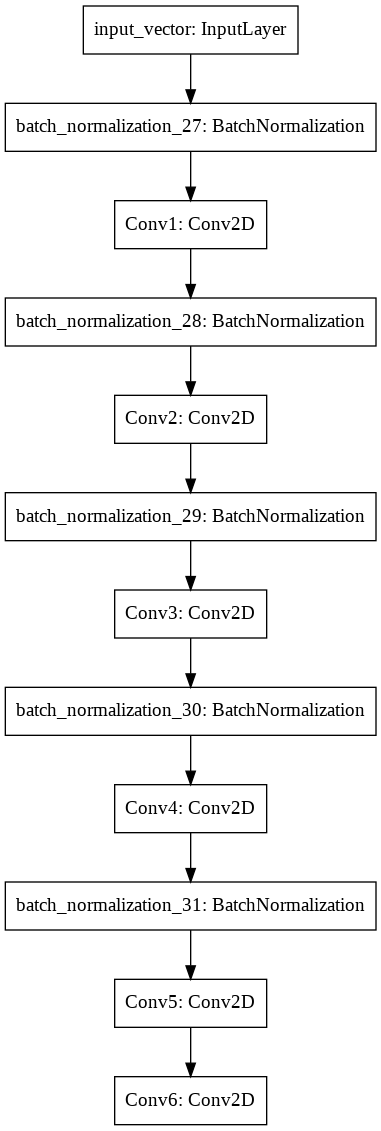
\includegraphics[width=100pt]{images/stacker.png}
    \caption{Sequence diagram of CNN stacker}
    \label{fig:stacker}
\end{figure}


    Figure \ref{fig:stacker} shows the sequence diagram of the 
    CNN stacker. It consists of 6 convolutional layers, with batch normalization applied before each layer, except for the last layer.

    Batch normalization are used with the aim to improve the performance, speed and stability of the model. The values from previous layer are normalized by subtracting the batch mean and dividing the batch standard deviation. The normalization reduces covariance shift and allows each layer in the model to learn more independently.
    
    Similar to the autoencoder, ReLU activation function is used to contain non-linearity in the model. For the last layer, sigmoid activation is used to predict pixel intensities between 1 and 0.
%------------------------------------------------------------------------
\section{Results}

\subsection{Autoencoder}

The autoencoder removes most of the background noise as shown in Figure \ref{fig:autoencoder} . The area of the stain becomes invisible while the texts can be clearly seen.
\begin{figure}[h!]
    \centering
    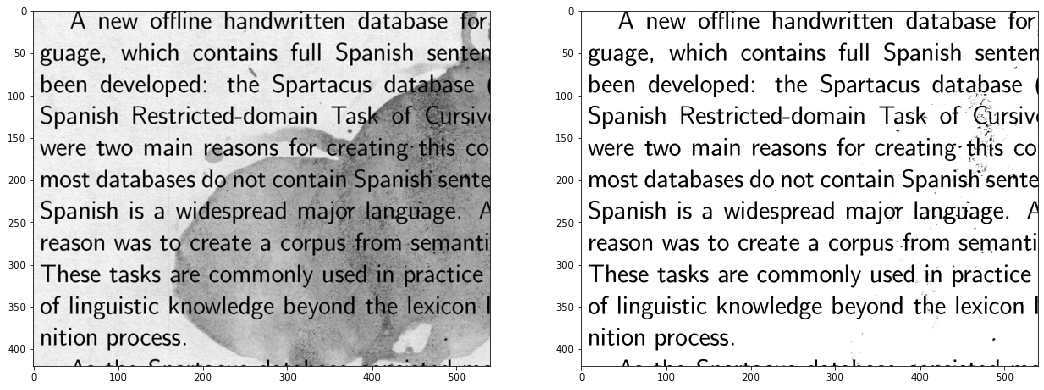
\includegraphics[width=\columnwidth]{images/autoencoder.png}
    \caption{Autoencoder output}
    \label{fig:autoencoder}
\end{figure}

Figure \ref{fig:autoencoderloss} shows the training and validation loss of the autoencoder model. We applied early stopping to prevent overfitting of training data. The best model was obtained at epoch 29 with 5 epochs of patience.

\begin{figure}[h!]
    \centering
    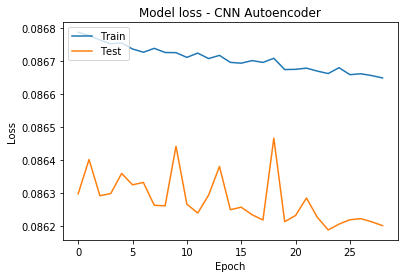
\includegraphics[width=\columnwidth]{images/autoencoder_loss.png}
    \caption{Training and Validation loss}
    \label{fig:autoencoderloss}
\end{figure}


\subsection{Median Filtering}
\begin{figure}[h!]
    \centering
    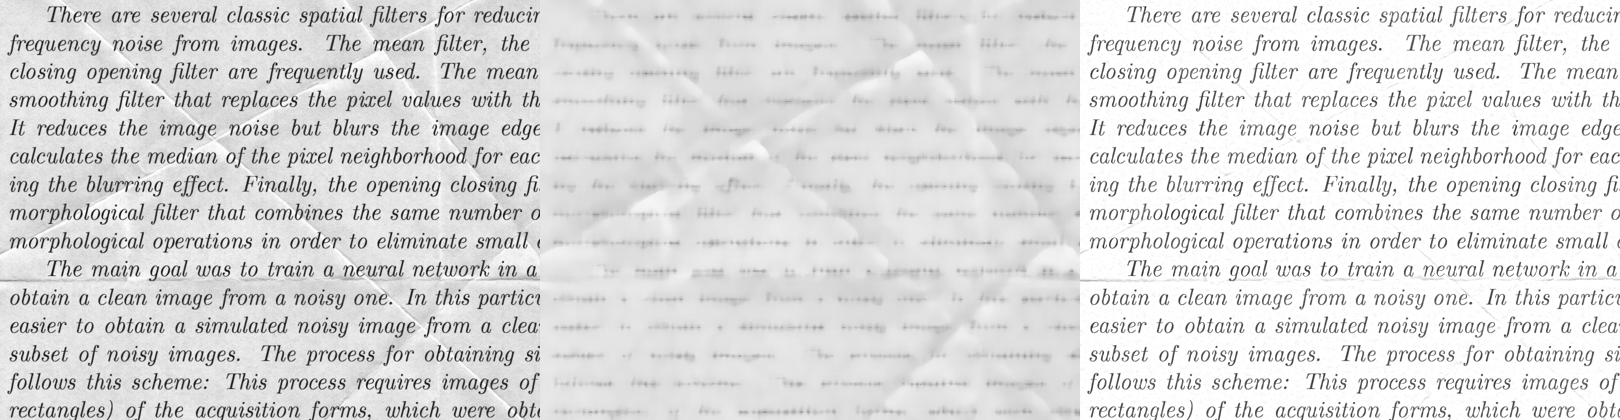
\includegraphics[width=\columnwidth]{images/median.png}
    \caption{Median filtering output}
    \label{fig:median}
\end{figure}
Median filtering was applied to filter the background noise as shown in the middle image in Figure \ref{fig:median}. The background noise is then used to be subtracted from the original image to obtain a clean image as shown in the right image in Figure \ref{fig:median}.


\subsection{Edge Detection, Erosion, Dilation}
\begin{figure}[h!]
    \centering
    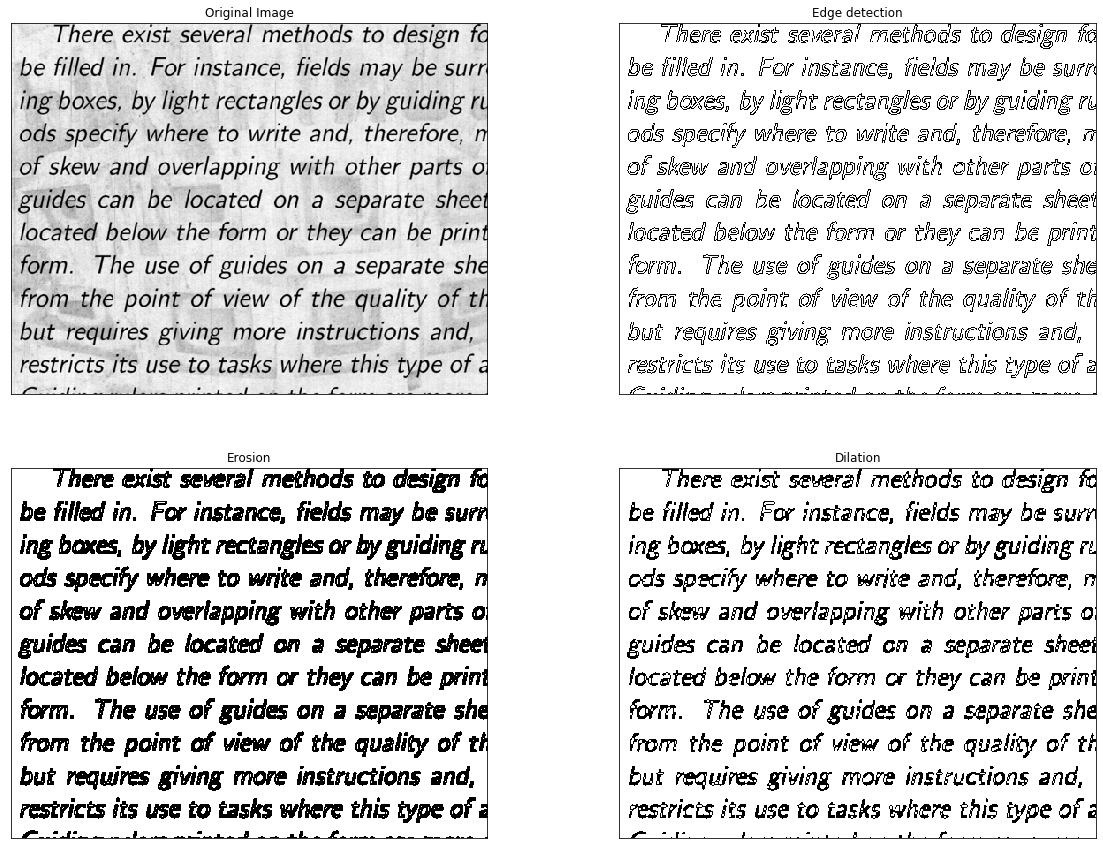
\includegraphics[width=\columnwidth]{images/edde.png}
    \caption{Edge detection, erosion, dilation}
    \label{fig:edde}
\end{figure}
Figure \ref{fig:edde} shows the original image, the images after applying edge detection, erosion and dilation. Edge detection removes most of the background noise while preserving the edges of the texts. Erosion makes edges thicker and dilation reverses the process to completely remove the background noise.


\subsection{Adaptive Thresholding}
\begin{figure}[h!]
    \centering
    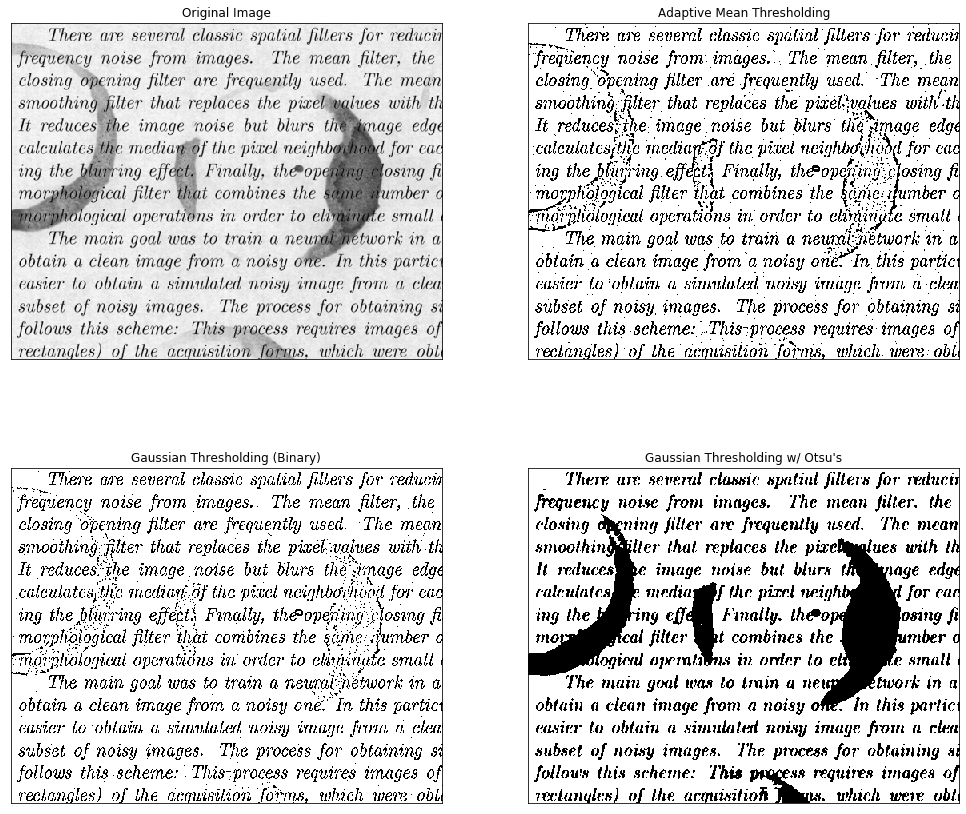
\includegraphics[width=\columnwidth]{images/thresholding.png}
    \caption{Adaptive thresholding output}
    \label{fig:thresholding}
\end{figure}
Figure \ref{fig:thresholding} shows different types of thresholding methods applied to a contaminated image. Gaussian Thresholding with Otsu's thresholding preserves the stains, which is the most undersired output. Adaptive mean thresholding only removes some parts of the stain area, while binary Gaussian thresholding performs the best by removing most of the stains and outputs the clearest image.

\subsection{Stacker}
\begin{figure}[h!]
    \centering
    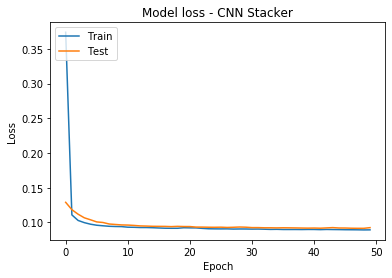
\includegraphics[width=\columnwidth]{images/stacker_loss_new.png}
    \caption{Training and Validation loss for CNN Stacker}
    \label{fig:stacker_loss}
\end{figure}

The stacker was able to effectively produce cleaner images of text given inputs from the 4 previous channels in addition to the original input image.However, its validation loss (0.0926) could not be minimized to be less than that of the CNN Autoencoder when run on its own (0.0862).

Similarly to the Autoencoder, training for the stacker was run using early stopping with a patience of 5 epochs. Figure \ref{fig:stacker_loss} shows the Training \& Validation Model loss for the CNN Stacker. Notice that unlike the same plot for the Autoencoder, the Validation loss for the CNN Stacker is consistently higher than the Training loss. Additionally, the minimum loss is greater than that of the autoencoder.

Finally, Figure \ref{fig:stacker_out} shows a selection of outputs from the final ensemble model from the test image set.

\begin{figure}[h]
    \centering
    \begin{subfigure}[b]{\columnwidth}
        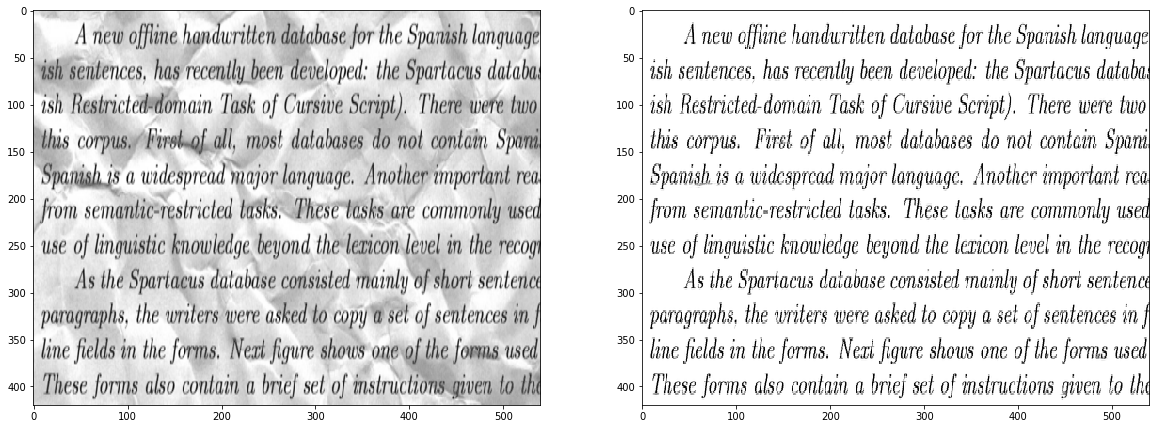
\includegraphics[width=\columnwidth]{images/stacker1.png}
    \end{subfigure}
    \begin{subfigure}[b]{\columnwidth}
        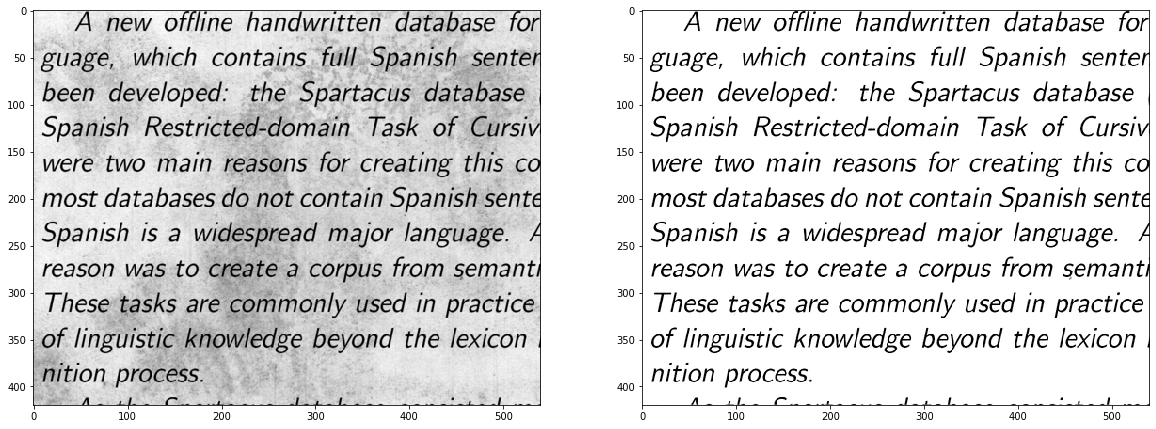
\includegraphics[width=\columnwidth]{images/stacker2.png}
    \end{subfigure}
    \begin{subfigure}[b]{\columnwidth}
        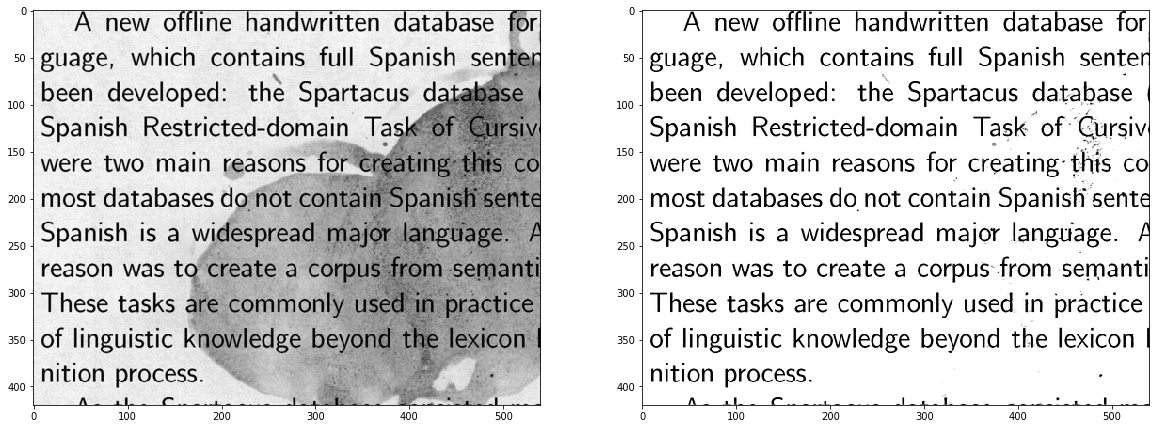
\includegraphics[width=\columnwidth]{images/stacker3.png}
    \end{subfigure}
    \begin{subfigure}[b]{\columnwidth}
        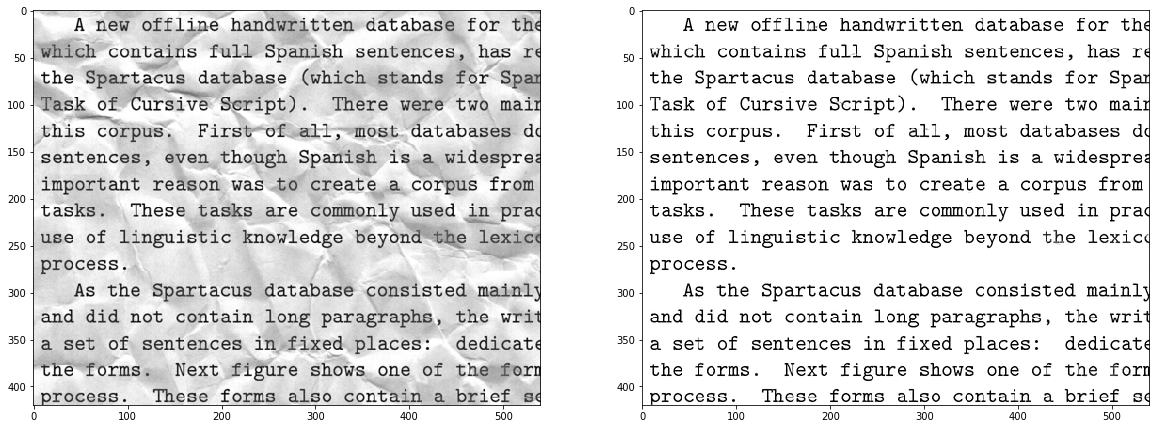
\includegraphics[width=\columnwidth]{images/stacker4.png}
    \end{subfigure}
    \caption{Assorted CNN stacker outputs from completed ensember model}
    \label{fig:stacker_out}
\end{figure}


%------------------------------------------------------------------------
\section{Conclusion}

By stacking the models together, we were able to achieve a decent performance from the stacker model. The outputs generated from the model are much more readable than the original images, as seen in the test outputs from the final ensemble model in Figure \ref{fig:stacker_out}. This offers a way to process images of documents to help enhance text seen in a photograph or to pre-process inputs to increase the efficacy of optical character recognition programs. This could also be implemented in consumer and business products such as mobile apps for document scanning as an improvement over today's approach of simply making basic photo adjustments to an image such as contrast, brightness, and saturation.

There is likely room for improvement over the models produced in this project, as further calibration of the stacker and autoencoder architectures should lead to a greater improvement in error by the former over the latter, which we were unable to achieve here.

Conversely, there is also the possibility that this problem is better suited to a single-CNN architecture solution and that an ensemble model may yield diminishing returns, which could explain our difficulties in finding significantly improved results from an ensemble model over a single model.

%------------------------------------------------------------------------



{\small
\bibliographystyle{ieee_fullname}
\bibliography{egbib}
}

\end{document}
